\documentclass[UTF8,ctexart,a4paper,11pt,openany]{article}
\usepackage[slantfont,boldfont]{xeCJK}
\usepackage{fontspec}
\usepackage{ctex}
\usepackage{booktabs}
\setCJKmainfont{SimSun}%[BoldFont=SimHei] %去掉注释:bf字体为黑体

\setsansfont{SimHei}
\setCJKsansfont{SimHei}

\xeCJKsetcharclass{"2160}{"2470}{1}% 1: CJK
\xeCJKsetup{AutoFallBack=true}
\setCJKfallbackfamilyfont{\CJKrmdefault}{SimSun.ttf}

%\setmainfont{Times New Roman}     %去掉注释:Times new roman字体
%\usepackage{mathptmx}             %去掉注释:Times new roman字体

\usepackage{mathtools}
\usepackage{amsmath}
\usepackage{amsfonts}
\usepackage{amssymb}
\usepackage{amsthm}
\usepackage[T1]{fontenc}
\usepackage{indentfirst} %段首空两格

\usepackage{graphicx}
\usepackage{geometry}
\usepackage{latexsym}
\usepackage{fancyhdr}
\usepackage{epstopdf}
%\usepackage{pifont}
%\usepackage[perpage,symbol*]{footmisc}
\usepackage{titlesec}
\usepackage{setspace}
\usepackage{enumerate}
\usepackage{enumitem}
\usepackage{multicol}
\usepackage{url}
\usepackage{exscale}
\usepackage{ulem}
\usepackage{relsize}
\usepackage{mathrsfs}
\usepackage{tikz}
\usepackage{wrapfig}
\usepackage{framed}
\usepackage{bm}
%\usepackage{pstricks,pst-node,multido,ifthen,calc}
\usepackage[all]{xy}
\usepackage{extarrows}
%\usepackage[backref]{hyperref}
\usepackage{hyperref}
\usepackage{stfloats} %插图的时候不分页

\setlength{\parindent}{2em} %段首空两格
\linespread{1.2}
\usepackage{listings}
\usepackage{xcolor}
\usepackage{algorithm}
\usepackage{algorithmicx}
\usepackage{algpseudocode}
\usepackage{mdframed}
\usepackage{extarrows}
\usepackage{diagbox}
\usepackage{makecell}

\theoremstyle{definition}
\mdfdefinestyle{theoremstyle}{%
linecolor=green!40,linewidth=.5pt,%
backgroundcolor=green!10,
skipabove=8pt,
skipbelow=5pt,
innerleftmargin=7pt,
innerrightmargin=7pt,
frametitlerule=true,%
frametitlerulewidth=.5pt,
frametitlebackgroundcolor=green!35,
frametitleaboveskip=0pt,
frametitlebelowskip=0pt,
innertopmargin=.4\baselineskip,
innerbottommargin=.4\baselineskip,
shadow=true,shadowsize=3pt,shadowcolor=black!20,
%theoremseparator={\hspace{1pt}},
theoremseparator={.},
nobreak=true,
}


\everymath{\displaystyle}

\newtheorem{definition}{\hspace{2em}定义}[section]
\newtheorem{axiom}{\hspace{2em}公理}

\mdtheorem[style=theoremstyle]{theorem}{定理}
\mdtheorem[style=theoremstyle]{example}{例}
\mdtheorem[style=theoremstyle]{exercise}{问题}
\newtheorem{lemma}[theorem]{\hspace{2em}引理}
\newtheorem{corollary}[theorem]{\hspace{2em}推论}

\newcommand*{\QED}{\hfill\ensuremath{\square}}
\newcommand*{\rmk}{\textbf{注:}}
\renewcommand*{\proof}{\textbf{证明:}}
\newcommand*{\tips}{\textbf{提示:}}
\newcommand*{\hard}{\textbf{\color{red}(难)}}
\newcommand*{\eqsmall}{\setlength\abovedisplayskip{1pt}\setlength\belowdisplayskip{1pt}}
\geometry{left=2cm,right=2cm,top=2cm,bottom=2cm}
% \title{数值分析上机报告(示例}
% \author{Fiddie}
\pagestyle{fancy}
\fancyfoot[C]{}
\fancyhead[RO]{ \thepage}
\fancyhead[LE]{\thepage  }
% \fancyhead[RE]{\rightmark (By Fiddie)}
% \fancyhead[LO]{\leftmark (By Fiddie)}
\titleformat{\chapter}{\centering\huge\bfseries}{第\,\thechapter\,章}{1em}{} %更改标题样式
\titleformat{\section}{\bfseries\Large}{$\S$\,\thesection\,}{1em}{} %更改标题样式
\titlespacing*{\chapter}{0pt}{9pt}{0pt} %调整标题间距
\setenumerate[1]{itemsep=0pt,partopsep=0pt,parsep=\parskip,topsep=0pt} %设置enumerate行间距
\setenumerate[2]{itemsep=0pt,partopsep=0pt,parsep=\parskip,topsep=0pt} %设置enumerate行间距
\setitemize[1]{itemsep=0pt,partopsep=0pt,parsep=\parskip,topsep=0pt} % 设置itemize行间距
\setlist[enumerate,2]{label=(\arabic*),topsep=0mm,itemsep=0mm,partopsep=0mm,parsep=\parskip}
    % 设置二层枚举为(1)样式
    
\newfontfamily\hei{SimHei}
\newcommand\textcf[1]{\textbf{\textsf{\hei{#1}}}}

\newcommand\e{\leftarrow}
%\renewcommand{\bibname}{参考文献}

\begin{document}
\begin{center}
{\huge \textbf{数值分析第9次上机作业}}

{\large 学号:221840189,姓名:王晨光}
\end{center}

\section{问题}
    常微分方程初值问题:$$\left\{\begin{array}{l}y^{\prime}=-\frac{1}{x^{2}}-\frac{y}{x}-y^{2}, \quad 1 \leq x \leq 2, \\ y(1)=-1 .\end{array}\right.$$

    \subsection{问题一}
    分别用 Euler 方法、改进的 Euler 方法、Heun 公式、中点方法和四阶 Runge-Kutta 方法求解上述初值问题,列表、画图比较他们的计算结果.

        \subsubsection{算法思路}

        根据插值型数值微分的思想,我们可以利用精确解在当前步和前几步的值做插值多项式, 再用其导数近似初值问题的导数得到数值方法,这样构造的方法称为BDF ( Backward differential formula) 方法(也称为 Gear 方法)。\par

        下面我们考虑如何利用前面介绍的函数插值法或者数值积分方法设计微分方程的离散化方法. 首先对微分方程$y^{\prime}=f(t,y)$在区间$[t_n,t_{n+1}]$上求积分得:$$y\left(t_{n+1}\right)-y\left(t_{n}\right)=\int_{t_{n}}^{t_{n+1}} f(t, y(t)) d t$$把$f(t,y(t))$换成它的插值多项式,或对右端积分使用数值积分公式, 我们将得到解初值问题的数值方法. 例如应用矩形公式:$$\int_{t_{n}}^{t_{n+1}} f(t, y(t)) d t \simeq h f\left(t_{n}, y\left(t_{n}\right)\right)$$再用$y_n$代替$y(t_n)$,便得到 Euler 方法:$$\begin{array}{c}y_{n+1}=y_{n}+h f\left(t_{n}, y_{n}\right), n=0,1,2, \cdots, N-1, \\ y_{0}=\eta .\end{array}$$ 仿照这样的思想,我们可以得到更多更精确的微分方程$\left\{\begin{array}{l}y^{\prime}(x)=f(x, y), \\ y(x_0)=y_0 .\end{array}\right.$数值解的公式:

        \begin{enumerate}
            \item 改进的 Euler 公式:$$\left\{\begin{array}{l}c_{1}=c_{2}=1 / 2 \\ a_{2}=1\end{array} \Rightarrow\left\{\begin{array}{l}y_{n+1}=y_{n}+h / 2\left[K_{1}+K_{2}\right] \\ K_{1}=f\left(x_{n}, y_{n}\right) \\ K_{2}=f\left(x_{n}+h, y_{n}+h K_{1}\right)\end{array}\right.\right.$$
            
            \item Heun 公式:$$\begin{array}{l}\left\{\begin{array}{l}c_{1}=1 / 4, c_{2}=3 / 4 \\ a_{2}=2 / 3\end{array}\right. \\ y_{n+1}=y_{n}+\frac{1}{4} h\left(K_{1}+3 K_{2}\right), n=0,1, \cdots, N-1\end{array}$$其中:$$\begin{array}{l}K_{1}=f\left(x_{n}, y_{n}\right), \\ K_{2}=f\left(x_{n}+\frac{2}{3} h, y_{n}+\frac{2}{3} h K_{1}\right), \\ y_{0}=\eta,\end{array}$$
            
            \item 中点方法:$$\begin{array}{l}\left\{\begin{array}{l}c_{1}=0, c_{2}=1 \\ a_{2}=1 / 2\end{array}\right. \\ y_{n+1}=y_{n}+h K_{2}, n=0,1, \cdots, N-1\end{array}$$其中:$$\begin{array}{l}K_{1}=f\left(x_{n}, y_{n}\right) \\ K_{2}=f\left(x_{n}+\frac{h}{2}, y_{n}+\frac{1}{2} h K_{1}\right) \\ y_{0}=\eta\end{array}$$

            \item 四阶 Runge-Kutta 方法:$$y_{n+1}=y_{n}+\frac{h}{6}\left(K_{1}+2 K_{2}+2 K_{3}+K_{4}\right), n=0,1, \cdots, N-1$$其中:$$\begin{array}{l}K_{1}=f\left(x_{n}, y_{n}\right), \\ K_{2}=f\left(x_{n}+\frac{1}{2} h, y_{n}+\frac{1}{2} h K_{1}\right), \\ K_{3}=f\left(x_{n}+\frac{1}{2} h, y_{n}+\frac{1}{2} h K_{2}\right), \\ K_{4}=f\left(x_{n}+h, y_{n}+h K_{3}\right), \\ y_{0}=\eta .\end{array}$$
             
        \end{enumerate}
        \subsubsection{结果分析}%重点(误差图、结果图、分析算法的收敛性(速度)、内存使用(时间、空间)、计算量、稳定性
        为了更显著地比较不同方法的效果,统一规定所有方法的步长$h=0.1$,即将区间$[1, 2]$划分为10个. \par
        
        将使用 python 中 scipy 库中的integrate.solve\_ivp函数求解得到的结果作为该初值问题的精确解,并与五种方法得到的结果进行比较. \par
        \begin{figure}[H]
            \centering
            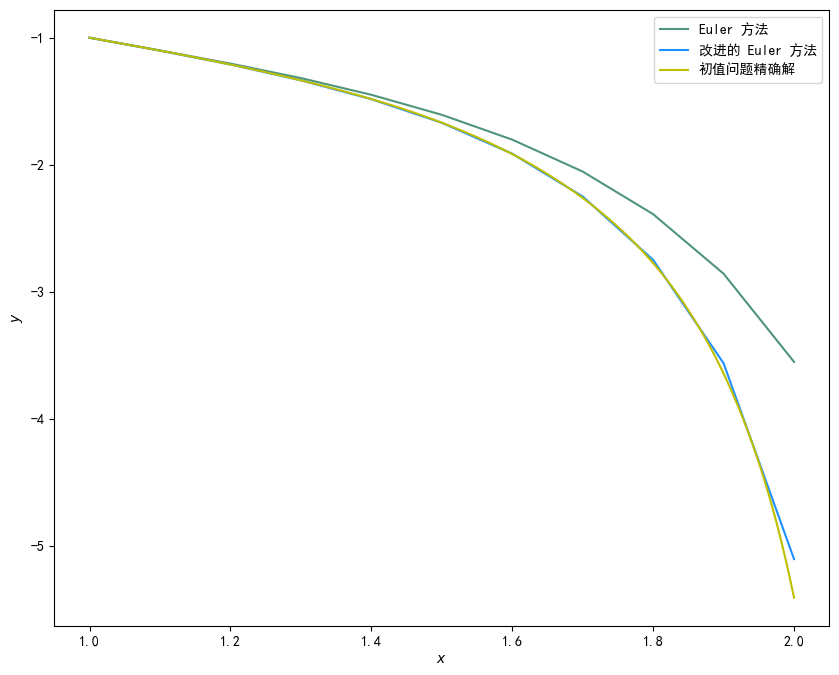
\includegraphics[width=0.45\linewidth]{pics/P9.1.png}
            \caption{Euler 方法的改进效果}
        \end{figure}

        可见在 Euler 方法基础上的改进给了算法很大的提升. \par

        \begin{figure}[H]
            \begin{minipage}{0.42\textwidth}
                \centering
                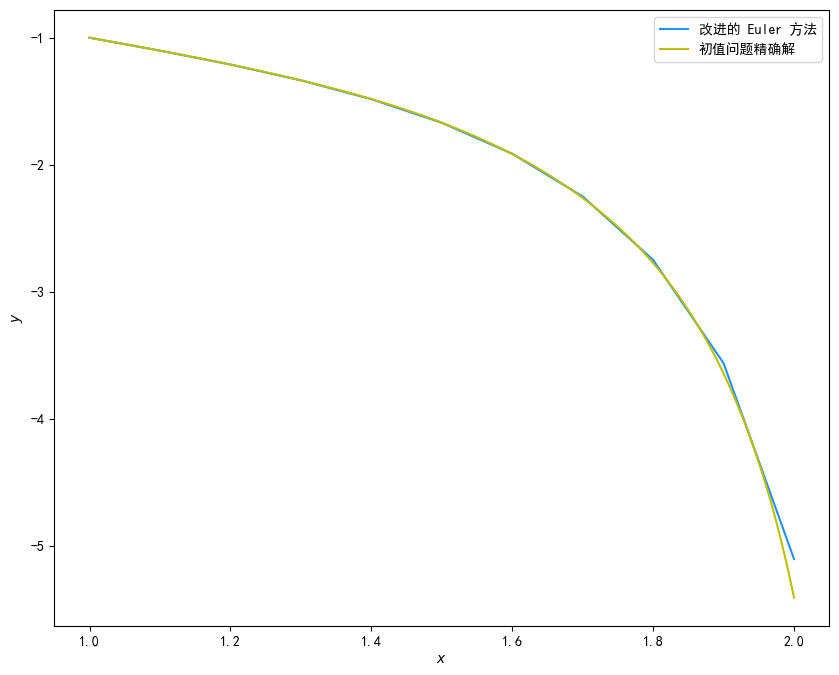
\includegraphics[width=\linewidth]{pics/P9.2.png}
            \end{minipage}%
            \hspace{2cm}
            \begin{minipage}{0.42\textwidth}
                \centering
                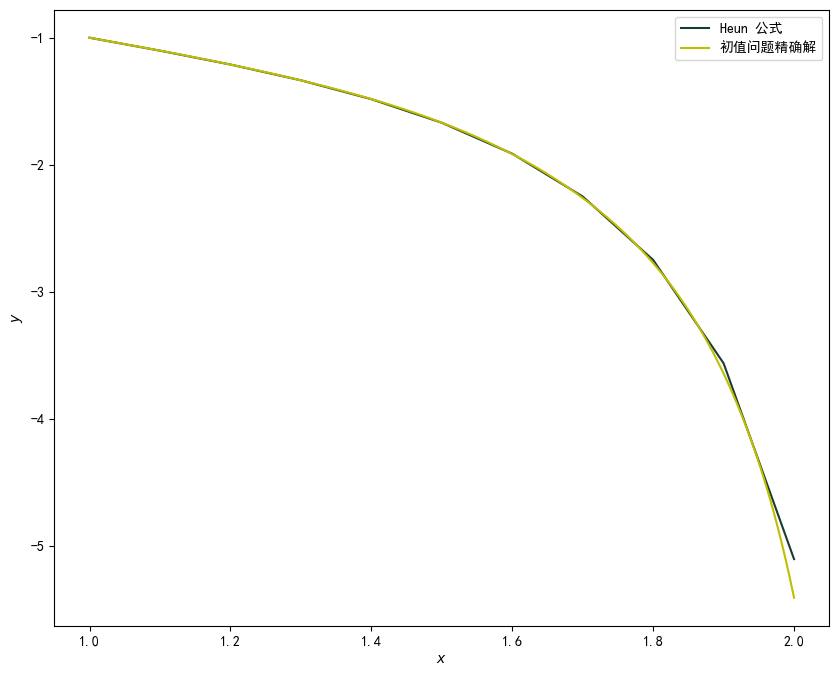
\includegraphics[width=\linewidth]{pics/P9.3.png}
            \end{minipage}%
            \\
            \begin{minipage}{0.42\textwidth}
                \centering
                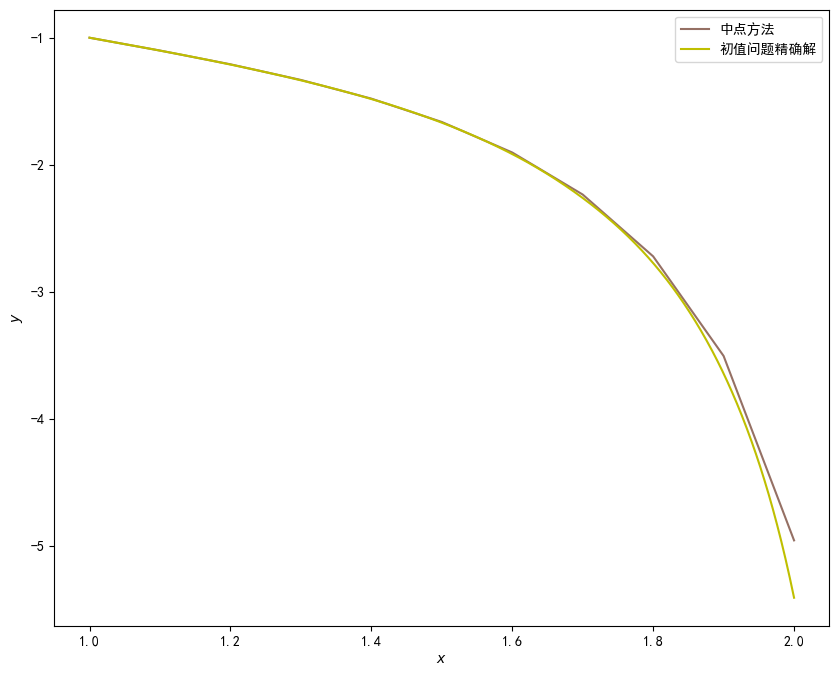
\includegraphics[width=\linewidth]{pics/P9.4.png}
            \end{minipage}
            \hspace{2cm}
            \begin{minipage}{0.42\textwidth}
                \centering
                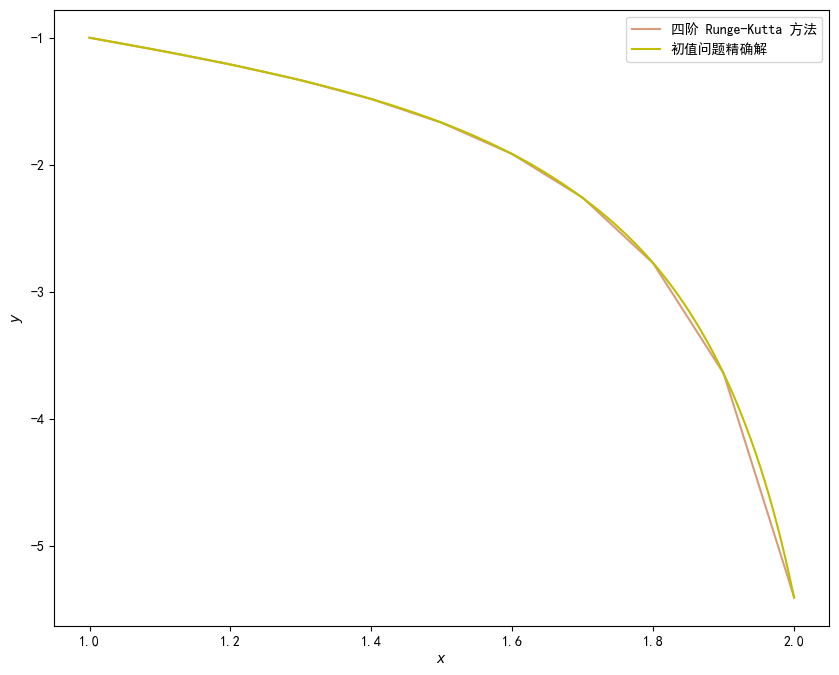
\includegraphics[width=\linewidth]{pics/P9.5.png}
            \end{minipage}
            \caption{结果比较}
        \end{figure}

        可见这四种方法在这个问题上面都有不错的使用效果. \par

\begin{table}[H]
	\centering
    \resizebox{\textwidth}{!}{%
	\begin{tabular}{ccccccc}
		\toprule
		$x$   & $y$                   & Euler               & Improved Euler      & Heun                & Midpoint            & 4-order Runge-Kutta \\ \midrule
		1.0 & -1.0                & -1.0                & -1.0                & -1.0                & -1.0                & -1.0                \\
		1.1 & -1.101282248845198  & -1.1                & -1.1018223140495869 & -1.1018223140495869 & -1.1009529478458049 & -1.1012826678659193 \\
		1.2 & -1.2110433325930738 & -1.2036446280991737 & -1.2109329616626514 & -1.2109329616626514 & -1.2092239073203017 & -1.2100751453889105 \\
		1.3 & -1.335157166350982  & -1.3176613926105536 & -1.3350267950205723 & -1.3350267950205723 & -1.3323361028616876 & -1.3340877915750706 \\
		1.4 & -1.482415949857855  & -1.4490975761389777 & -1.4834058063949158 & -1.4834058063949158 & -1.479385598657663  & -1.482749368299053  \\
		1.5 & -1.6684358216956912 & -1.6065993930952163 & -1.6691140645680864 & -1.6691140645680864 & -1.6630840854650728 & -1.6694425780891586 \\
		1.6 & -1.915656859375965  & -1.8020533723227048 & -1.9126352193216483 & -1.9126352193216483 & -1.9032722875944785 & -1.9154952225080968 \\
		1.7 & -2.26116559591342   & -2.053227172222499  & -2.249514782136032  & -2.249514782136032  & -2.234074247576292  & -2.2586983818103605 \\
		1.8 & -2.7733458410437857 & -2.388625361468082  & -2.7484745656328373 & -2.7484745656328373 & -2.720602215799331  & -2.774579055172638  \\
		1.9 & -3.642936111981181  & -2.8573412617733496 & -3.5620301560265935 & -3.5620301560265935 & -3.5044281499982297 & -3.640916010383189  \\
		2.0 & -5.40707572282345   & -3.551095619222935  & -5.103210160551191  & -5.103210160551191  & -4.955788578459564  & -5.400991565128523  \\ \bottomrule
	\end{tabular}
    }
	\caption{五种方法在插值基点上的取值与精确值的比较}
\end{table}

    可以看出除了四阶 Runge-Kutta 方法,其他方法的误差都有增大的趋势,这个现象在$x=2$处可以直观地看出. 

    \subsection{问题二} 

        用经典的 Runge-Kutta 方法提供初始出发值,与四阶 Adams 预测-校正方法的 PECE 模式结合起来求解上述初值问题,并与 (1) 中的四阶 Runge-Kutta 方法求解进行比较.

        \subsubsection{算法思路}

        预测公式:$$y_{n+1}^{(0)}=y_{n}+\frac{n}{24}\left[55 f_{n}-59 f_{n-1}+37 f_{n-2}-9 f_{n-3}\right]$$校正公式:$$y_{n+1}=y_{n}+\frac{h}{24}\left[9 f_{n+1}^{(0)}+19 f_{n}-5 f_{n-1}+f_{n-2}\right]$$其 PECE 模式为:$$\begin{array}{ll}P: & y_{n+1}^{(0)}=y_{n}+\frac{h}{24}\left[55 f_{n}-59 f_{n-1}+37 f_{n-2}-9 f_{n-3}\right] \\ E: & f_{n+1}^{(0)}=f\left(t_{n+1}, y_{n+1}^{(0)}\right) \\ C: & y_{n+1}=y_{n}+\frac{h}{24}\left(9 f^{(0)}{ }_{n+1}+19 f_{n}-5 f_{n-1}+f_{n-2}\right) \\ E: & f_{n+1}=f\left(t_{n+1}, y_{n+1}\right)\end{array}$$其中用P表示预测过程. C表示校正过程, E表示计算$f$的过程. 

        \subsubsection{结果分析}
        \begin{figure}[H]
            \centering
            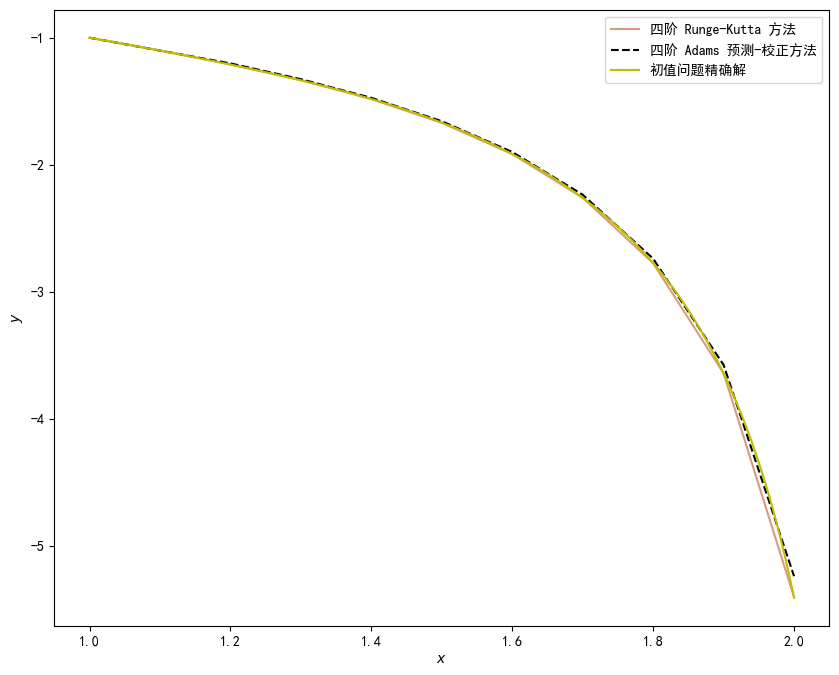
\includegraphics[width=0.45\linewidth]{pics/P9.6.png}
            \caption{结果比较}
            \end{figure}
        
            可见如果仅仅使用极少数的 Runge-Kutta 方法提供的初始点, 四阶 Adams 预测-校正方法的 PECE 模式就会有较不错的表现, 但最终的效果不如完全使用四阶 Runge-Kutta 方法. 尤其是在$x=2$处, 这在下表中也可以明显地看出: 

        \begin{table}[H]
            \centering
            % \resizebox{\textwidth}{!}{%
            \begin{tabular}{cccc}
                \toprule
                $x$   & $y$                   & 4-order Runge-Kutta & 4-order Adams       \\ \midrule
                1.0 & -1.0                & -1.0                & -1.0                \\
                1.1 & -1.101282248845198  & -1.1012826678659193 & -1.1012826678659193 \\
                1.2 & -1.2110433325930738 & -1.2100751453889105 & -1.2018351932142624 \\
                1.3 & -1.335157166350982  & -1.3340877915750706 & -1.3261530760597708 \\
                1.4 & -1.482415949857855  & -1.482749368299053  & -1.4732204768780879 \\
                1.5 & -1.6684358216956912 & -1.6694425780891586 & -1.6572302727892014 \\
                1.6 & -1.915656859375965  & -1.9154952225080968 & -1.8991814924893602 \\
                1.7 & -2.26116559591342   & -2.2586983818103605 & -2.2355054775965906 \\
                1.8 & -2.7733458410437857 & -2.774579055172638  & -2.7384415918600347 \\
                1.9 & -3.642936111981181  & -3.640916010383189  & -3.5752795942449733 \\
                2.0 & -5.40707572282345   & -5.400991565128523  & -5.2377466864277435 \\ \bottomrule
            \end{tabular}
            %}
            \caption{两种方法在插值基点上的取值与精确值的比较}
        \end{table}
\section{结论}

        如果只从计算结果精确度来看, 四种解微分方程数值解的方法中, 无改进的 Euler 方法效果最差, 四阶 Runge-Kutta 方法和与之结合的四阶 Adams 预测-校正方法的 PECE 模式效果最好, 改进的 Euler 方法、Heun 公式、中点方法也都有着不错的效果. 
\clearpage

\section{附录: 程序代码}
\lstset{
    numbers=left,
    language=Python,
    keywordstyle=\color{blue!100},
    commentstyle=\color{green!50!blue!50!},
    frame=shadowbox,%阴影
    escapeinside='',%英文分号输入中文
    xleftmargin=2em,xrightmargin=2em,aboveskip=1em,
    framexleftmargin=2em,
    extendedchars=false}

\begin{lstlisting}[aboveskip=0pt]
import numpy as np
import matplotlib.pyplot as plt
# 定义常微分方程
def f(x, y):
    return -1/x**2 - y/x - y**2

# 定义各数值方法
def euler_method(f, x0, y0, h, n):
    x = np.zeros(n+1)
    y = np.zeros(n+1)
    x[0] = x0
    y[0] = y0
    for i in range(n):
        y[i+1] = y[i] + h * f(x[i], y[i])
        x[i+1] = x[i] + h
    return x, y

def improved_euler_method(f, x0, y0, h, n):
    x = np.zeros(n+1)
    y = np.zeros(n+1)
    x[0] = x0
    y[0] = y0
    for i in range(n):
        x[i+1] = x[i] + h
    for i in range(n):
        y_star = y[i] + h * f(x[i], y[i])
        y[i+1] = y[i] + h/2 * (f(x[i], y[i]) + f(x[i+1], y_star))
    return x, y

def heun_method(f, x0, y0, h, n):
    x = np.zeros(n+1)
    y = np.zeros(n+1)
    x[0] = x0
    y[0] = y0
    for i in range(n):
        k1 = f(x[i], y[i])
        k2 = f(x[i] + h, y[i] + h * k1)
        y[i+1] = y[i] + h/2 * (k1 + k2)
        x[i+1] = x[i] + h
    return x, y

def midpoint_method(f, x0, y0, h, n):
    x = np.zeros(n+1)
    y = np.zeros(n+1)
    x[0] = x0
    y[0] = y0
    for i in range(n):
        k1 = f(x[i], y[i])
        k2 = f(x[i] + h/2, y[i] + h/2 * k1)
        y[i+1] = y[i] + h * k2
        x[i+1] = x[i] + h
    return x, y

def runge_kutta_4(f, x0, y0, h, n):
    x = np.zeros(n+1)
    y = np.zeros(n+1)
    x[0] = x0
    y[0] = y0
    for i in range(n):
        k1 = f(x[i], y[i])
        k2 = f(x[i] + h/2, y[i] + h/2 * k1)
        k3 = f(x[i] + h/2, y[i] + h/2 * k2)
        k4 = f(x[i] + h, y[i] + h * k3)
        y[i+1] = y[i] + h/6 * (k1 + 2*k2 + 2*k3 + k4)
        x[i+1] = x[i] + h
    return x, y

# 四阶 Adams 预测-校正方法
def adams_predictor_corrector(f, x0, y0, h, n):
    x = np.zeros(n+1)
    y = np.zeros(n+1)
    x_copy, y_copy = runge_kutta_4(f, x0, y0, h, 1)
    for i in range(2):
        x[i] = x_copy[i]
        y[i] = y_copy[i]
    for i in range(1, n):
        x[i+1] = x[i] + h
    for i in range(1, n):
        y_predict = y[i] + h/24 * (55*f(x[i], y[i]) - 59*f(x[i-1], y[i-1]) + 37*f(x[i-2], y[i-2]) - 9*f(x[i-3], y[i-3]))
        y_correct = y[i] + h/24 * (9*f(x[i+1], y_predict) + 19*f(x[i], y[i]) - 5*f(x[i-1], y[i-1]) + f(x[i-2], y[i-2]))
        y[i+1] = y_correct
    return x, y
# 初始条件和步长
x0, y0 = 1, -1
h = 0.1
n = int((2 - x0) / h)
# 求解
x_euler, y_euler = euler_method(f, x0, y0, h, n)
x_improved_euler, y_improved_euler = improved_euler_method(f, x0, y0, h, n)
x_heun, y_heun = heun_method(f, x0, y0, h, n)
x_midpoint, y_midpoint = midpoint_method(f, x0, y0, h, n)
x_rk4, y_rk4 = runge_kutta_4(f, x0, y0, h, n)
x_adams, y_adams = adams_predictor_corrector(f, x0, y0, h, n)
# 列表输出计算结果
# print("x values:", x_rk4)
# print("Euler Method:", y_euler)
# print("Improved Euler Method:", y_improved_euler)
# print("Heun Method:", y_heun)
# print("Midpoint Method:", y_midpoint)
print("Runge-Kutta 4 Method:", y_rk4)
print("Adams Predictor-Corrector Method:", y_adams)
from scipy.integrate import solve_ivp
x_span=(1, 2)
y_0=np.array([-1])
sol=solve_ivp(f, x_span, y_0, method='RK45', dense_output=True)
x_values = np.linspace(x_span[0], x_span[1], 1000)
y_values = sol.sol(x_values)
print("Solution: ", sol.sol(x_rk4)[0])
print("Runge-Kutta 4 Method:", y_rk4)
print("Adams Predictor-Corrector Method:", y_adams)
for i in range(11):
    # print(x_rk4[i])
    # print(y_euler[i])
    # print(y_improved_euler[i])
    # print(y_heun[i])
    # print(y_midpoint[i])

    # print(sol.sol(x_rk4)[0][i])
    # print(y_rk4[i])
    print(y_adams[i])
# 画图
plt.rcParams['font.sans-serif'] = ['SimHei']  # 指定默认字体
plt.rcParams['axes.unicode_minus'] = False
plt.figure(figsize=(10, 8))
# plt.plot(x_euler, y_euler, label='Euler 方法', color='#509579')
# plt.plot(x_improved_euler, y_improved_euler, label='改进的 Euler 方法', color='dodgerblue')
# plt.plot(x_heun, y_heun, label='Heun 公式', color='#1a3b30')
# plt.plot(x_midpoint, y_midpoint, label='中点方法', color='#957064')
plt.plot(x_rk4, y_rk4, label='四阶 Runge-Kutta 方法', color='#d89c7c')
plt.plot(x_adams, y_adams, label='四阶 Adams 预测-校正方法', color='black', linestyle='--')
plt.plot(x_values, y_values[0], label='初值问题精确解', color='y')
plt.xlabel('$x$')
plt.ylabel('$y$')
plt.legend()
plt.show()
    
\end{lstlisting}

\clearpage



\section{附录: 题目二程序代码}
\lstset{
    numbers=left,
    language=Python,
    keywordstyle=\color{blue!100},
    commentstyle=\color{green!50!blue!50!},
    frame=shadowbox,%阴影
    escapeinside='',%英文分号输入中文
    xleftmargin=2em,xrightmargin=2em,aboveskip=1em,
    framexleftmargin=2em,
    extendedchars=false}

\begin{lstlisting}[aboveskip=0pt]

\end{lstlisting}

\clearpage

\bibliographystyle{unsrt}
\bibliography{Reference}
\end{document}